\begin{frame}[fragile]{Aplicación:}{DynamoDB}
    \justifying

    Dynamo utiliza relojes vectoriales para mantener el control de versiones del
    objeto en varias réplicas. Un reloj vectorial es efectivamente una lista de
    pares (nodo, contador). Un reloj vectorial está asociado con cada versión de
    cada objeto.

    \begin{center}
        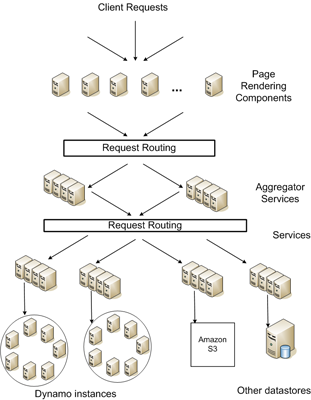
\includegraphics[scale=0.4]{D2.png}
        \end{center}

\end{frame}
